% Lecture file created by newnote
% Class: Models of Theoretical Physics
% Professor: Azaele Sandro
% Date: 2025-10-17
\lecture{7}{Wiener path integral}{2025-10-17}
\pagelayout{margin}
% --- Start writing here ---

\section{Wiener path integral}
The Wiener measure and the Wiener path integral (Techniques and Applications of Path Integration by L.S. Schulman)
We have seen that the propagator of the Brownian motion satisfies the Chapman-Kolmogorov eq. because it is a Markov process.
From eq. (13) and (11)
\begin{DispWithArrows}[tag=14]
    w\left(x_{2}, t_{2} \mid x_{0}, t_{0}\right)=\int_{-\infty}^{+\infty} w\left(x_{2}, t_{2} \mid x_{1}, t_{1}\right) w\left(x_{1}, t_{1} \mid x_{0}, t_{0}\right) d x_{1}
\end{DispWithArrows}
Notice the analogy with QM: $\left\langle x_{2} t_{2} \mid x_{0} t_{0}\right\rangle=w\left(x_{2} t_{2} \mid x_{0} t_{0}\right)$, we insert an identity $\int d x_{1}\left|x_{1}, t_{1}\right\rangle\left\langle x_{1}, t_{1}\right|=1$ and get $\left\langle x_{2} t_{2} \mid x_{0} t_{0}\right\rangle=\int d x_{1}\left\langle x_{2} t_{2} \mid x_{1} t_{1}\right\rangle\left\langle x_{1} t_{1} \mid x_{0} t_{0}\right\rangle$
We can also iterate eq. (14) $n$-times and get for $t_{n}>t_{n-1}>\ldots>t_{1}>t_{0}$
\begin{DispWithArrows}[tag=14b]
    w\left(x_{n}, t_{n} \mid x_{0}, t_{0}\right)=\int_{-\infty}^{+\infty} w\left(x_{n}, t_{n} \mid x_{n-1}, t_{n-1}\right) \cdots w\left(x_{1}, t_{1} \mid x_{0}, t_{0}\right) d x_{n-1} \cdots d x_{1}
\end{DispWithArrows}
This is an important property of the propagator, because it allows us to understand what is the probability to find a Brownian particle in different regions at different times. Indeed, if we define the Wiener measure $t_{n}>t_{n-1}>\ldots>t_{1}>t_{0}$
\begin{DispWithArrows}
    d \mathbb{P}_{t_{1} \ldots t_{n}}\left(x_{1} \ldots x_{n} \mid x_{0}, t_{0}\right)=\prod_{i=1}^{n} w\left(x_{i}, t_{i} \mid x_{i-1}, t_{i-1}\right) d x_{i}
\end{DispWithArrows}
then (interval $A_{i} \subseteq \mathbb{R}$)
\begin{DispWithArrows}[tag=15]
    \mathbb{P}\left(\{A\} \mid x_{0}, t_{0}\right) = \int_{A_{n}} \cdots \int_{A_{1}} w\left(x_{n} t_{n} \mid x_{n-1} t_{n-1}\right) \cdots w\left(x_{1} t_{1} \mid x_{0} t_{0}\right) d x_{n} \cdots d x_{1}
\end{DispWithArrows}
gives the joint probability to find a Brownian particle in the area $A_{1}$ at time $t_{1}$, within $A_{2}$ at time $t_{2}$ and within $A_{n}$ at time $t_{n}\left(t_{1}<t_{2} \cdots<t_{n}\right)$, given that it started off at $x_{0}$ at time $t_{0}<t_{1}$.
\begin{figure}[H]
    \centering
    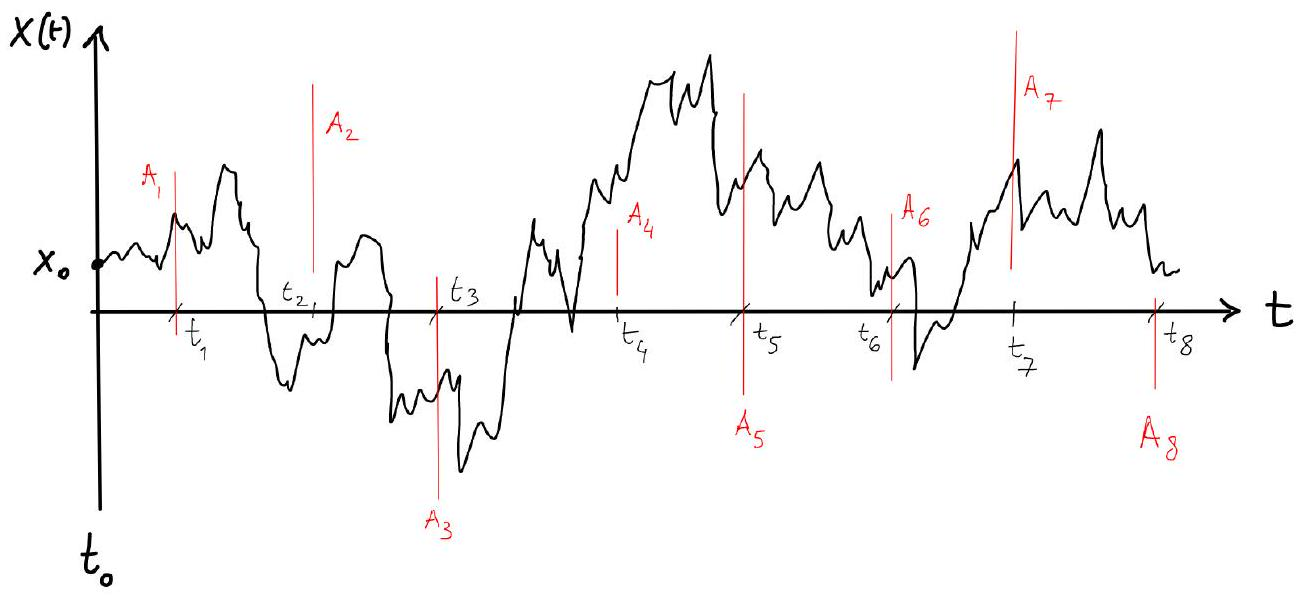
\includegraphics[width=\textwidth]{2025_10_17_55d6813539323d2293f0g-2}
\end{figure}
The explicit expression is $\left(\Delta t_{i}=t_{i}-t_{i-1}>0\right)$
\begin{DispWithArrows}[tag=16]
    d \mathbb{P}_{t_{1} \ldots t_{n}}\left(x_{1} \ldots x_{n} \mid x_{0}, t_{0}\right)=e^{-\frac{1}{2 D} \sum_{i=1}^{n} \frac{\left(x_{i}-x_{i-1}\right)^{2}}{\Delta t_{i}}} \prod_{i=1}^{n} \frac{d x_{i}}{\sqrt{2 \pi D \Delta t_{i}}}
\end{DispWithArrows}
This relation is valid for any $n \in \mathbb{N}$ and we can extend the result to any subset of the $\sigma$-algebra generated by the cylindrical sets of the form $A=\left\{x(t): x\left(t_{1}\right) \in A_{1}, x\left(t_{2}\right) \in A_{2} \ldots x\left(t_{n}\right) \in A_{n}\right\}$. When we take the limit $n \rightarrow \infty$ we obtain the so called Wiener path integral. In this case
\begin{DispWithArrows}
    \sum_{i=1}^{n} \frac{\left(x_{i}-x_{i-1}\right)^{2}}{\Delta t_{i}}=\sum_{i=1}^{n}\left(\frac{x_{i}-x_{i-1}}{\Delta t_{i}}\right)^{2} \Delta t_{i} \xrightarrow[\substack{n \to \infty \\ \max(\Delta t_i) \to 0}]{\sum \Delta t_i = T} \int_{0}^{T}(\dot{x}(s))^{2} d s
\end{DispWithArrows}
and eq. (16) gets the suggestive form
\begin{DispWithArrows}[tag=17]
    d \mathbb{P}_{w} \propto \prod_{\tau=0^{+}}^{T} d x(\tau) e^{-\frac{1}{2 D} \int_{0}^{T} \dot{x}(s)^{2} d s}
\end{DispWithArrows}
This formula is only formal as it does not exist (it is infinite!). However, it is very useful for calculating averages of functionals which are exponentials of quadratic expressions of the trajectory $x(s)$ or for approximations with the saddle point method.
Another way to look at eq. (14b) is the following. We fix $x_{n}=x$, $t_{n}=T$ and $x_{0}$ at $t_{0}$. Then all the integrations $x_{n-1}, x_{n-2} \ldots, x_{1}$ at the corresponding ordered times $t_{n-1}, \ldots t_{1}$ show that in the limit $n \rightarrow \infty$ (with fixed $x, T ; x_{0}, t_{0}$ ) the propagator of a Brownian particle $W\left(x, T \mid x_{0}, t_{0}\right)$ can be written as
\begin{DispWithArrows}[tag=17b]
    w\left(x, T \mid x_{0}, t_{0}\right)=\int_{x(0)=x_0}^{x(T)=x} \mathcal{D} x(\tau) e^{-\frac{1}{2 D} \int_{0}^{T} \dot{x}(s)^{2} d s}=\int_{x(0)=x_0}^{x(T)=x} \mathcal{D} x(\tau) e^{-S[x(s)]}
\end{DispWithArrows}
\begin{figure}[H]
    \centering
    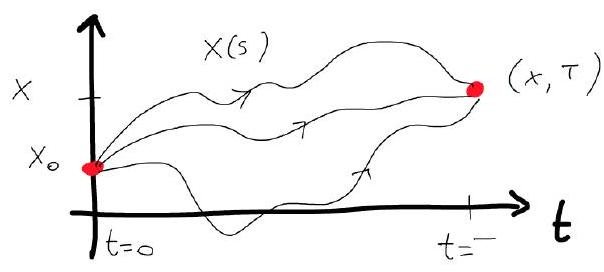
\includegraphics[width=\textwidth]{2025_10_17_55d6813539323d2293f0g-3}
\end{figure}
the propagator $W$ can be written as an integral over all trajectories between ($t_0, x_{0}$) and ($T, x$) of the Brownian particle.

Here $S[x(s)]$ is the action and $S=\int_{0}^{T} L[x] d s$, where $L$ is the Lagrangian of the system. Here $L[x(s)]=\frac{1}{2 D}\left(\frac{d x}{d s}\right)^{2}$ which can be interpreted as the kinetic energy of a free particle. Furthermore, notice that if we change variable $s=i t / \hbar$ (as an analytic continuation), identify $D=\frac{\hbar^{2}}{m}$ and introduce the "imaginary" time $\tilde{t}=-i \hbar T$, then the propagator in (17b) becomes
\begin{DispWithArrows}[tag=17c]
    W\left(x, \tilde{t} \mid x_{0}, 0\right)=\int_{x(0)=x_0}^{x(\tilde{t})=x} \mathcal{D} x\left(t^{\prime}\right) e^{\frac{i}{\hbar} \int_{0}^{\tilde{t}} \frac{1}{2} m\left(\frac{d x}{d t^{\prime}}\right)^{2} d t^{\prime}}=\sqrt{\frac{m}{2 \pi i \hbar \tilde{t}}} e^{\frac{i m}{2 \hbar \tilde{t}}\left(x-x_{0}\right)^{2}}
\end{DispWithArrows}
This is the propagator (or Green's function) of the Schrödinger eq:
\begin{DispWithArrows}
    i \hbar \frac{\partial \psi}{\partial t}=\hat{H} \psi \quad \text { where } \quad \hat{H}=-\frac{\hbar^{2}}{2 m} \frac{\partial^{2}}{\partial x^{2}}
\end{DispWithArrows}
we can write $W\left(x, \tilde{t} \mid x_{0}, 0\right)=\langle x| e^{-\frac{i}{\hbar} \tilde{t} \hat{H}}\left|x_{0}\right\rangle$
and correspondingly we can also write $\hat{H}|k\rangle=\frac{\hbar^{2}}{2 m} k^{2}|k\rangle=\frac{D k^{2}}{2}|k\rangle$
\begin{DispWithArrows}
    \begin{aligned}
    W\left(x, T \mid x_{0}, 0\right) & =\langle x| e^{-T H}\left|x_{0}\right\rangle=\int d k \int d k^{\prime}\left\langle x \mid k^{\prime}\right\rangle\left\langle k^{\prime}\right| e^{-T H}|k\rangle\langle k \mid x_0\rangle=\\\n    = & \frac{1}{2 \pi} \int d k e^{-\frac{D}{2} T k^{2}} e^{i k\left(x-x_{0}\right)}=\frac{1}{\sqrt{2 \pi D T}} e^{-\frac{\left(x-x_{0}\right)^{2}}{2 D T}} \quad\left\langle x \mid k^{\prime}\right\rangle=\frac{1}{\sqrt{2 \pi}} e^{i k^{\prime} x}
    \end{aligned}
\end{DispWithArrows}
This can be generalized to the case of $\hat{H}=-\frac{\hbar^{2}}{2 m} \frac{\partial^{2}}{\partial x^{2}}+V(x)$ (Schulman, Ch.9). Similar connections to statistical mechanics as $T \rightarrow \beta$ (Ch. 26).

\subsection*{Two-point correlation function (exercise)}
With the help of eq. (16) it is easy to calculate the 2-point correlation function which is defined as $\left\langle x\left(t_{1}\right) x\left(t_{2}\right)\right\rangle$ for $t_{0}<t_{1}<t_{2}$. We assume that the particle starts at $x_{0}=x\left(t_{0}\right)$.
\begin{figure}[H]
    \centering
    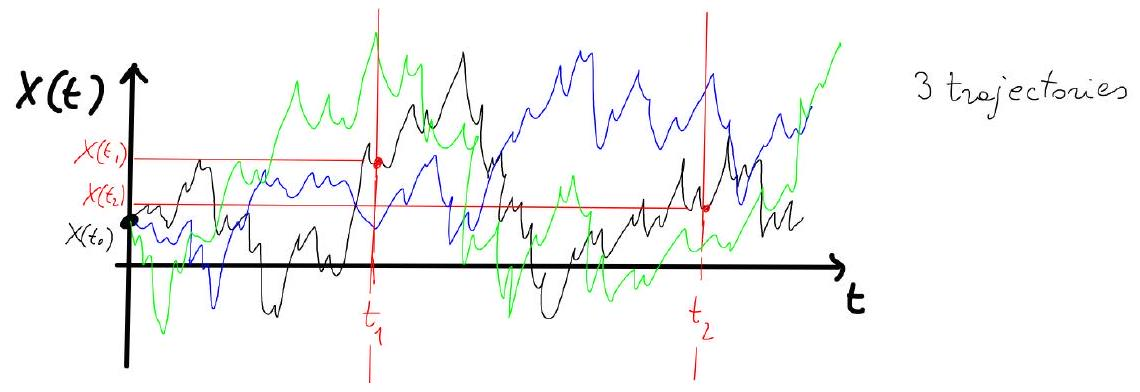
\includegraphics[width=\textwidth]{2025_10_17_55d6813539323d2293f0g-4}
\end{figure}
Average over Brownian trajectories, all starting at $x_{0}$ at time $t=t_{0}$, when looking at the trajectories at times $t=t_{1}$ and $t=t_{2}$.
\begin{DispWithArrows}[tag=18]
    \left\langle x\left(t_{1}\right) x\left(t_{2}\right)\right\rangle_{w}=\iint d \mathbb{P}_{t_{1} t_{2}}\left(x_{1}, x_{2} \mid x_{0}, t_{0}\right) x_{1} x_{2}
\end{DispWithArrows}
\begin{DispWithArrows}
    =\int_{-\infty}^{+\infty} d x_{2} \int_{-\infty}^{+\infty} d x_{1} \frac{1}{\sqrt{2 \pi D\left(t_{2}-t_{1}\right)}} e^{-\frac{1}{2 D} \frac{\left(x_{2}-x_{1}\right)^{2}}{t_{2}-t_{1}}} \frac{1}{\sqrt{2 \pi D\left(t_{1}-t_{0}\right)}} e^{-\frac{1}{2 D} \frac{\left(x_{1}-x_{0}\right)^{2}}{t_{1}-t_{0}}} x_{2} x_{1}
\end{DispWithArrows}
We change variables: $x=x_{1}-x_{0}, y=x_{2}-x_{1}$
\begin{DispWithArrows}
    x_{2}=x_{0}+x+y \quad x_{1}=x+x_{0} \quad\left(x_{0} \text { is a const. }\right)
\end{DispWithArrows}
Remember the Jacobian in the transformation:
\begin{DispWithArrows}
    p\left(x_{1}, x_{2}\right) d x_{1} d x_{2}=p\left(x_{1}(x, y), x_{2}(x, y)\right)|J| d x d y \\
    J=\left(\begin{array}{cc}
    \frac{\partial x_{1}}{\partial x} & \frac{\partial x_{1}}{\partial y} \\
    \frac{\partial x_{2}}{\partial x} & \frac{\partial x_{2}}{\partial y}
\end{array}\right)=\left(\begin{array}{cc}1 & 0 \\ 1 & 1\end{array}\right) \Rightarrow|J|=1
\end{DispWithArrows}
From eq. (18) we get
\begin{DispWithArrows}
    \begin{aligned}
    & =\int_{-\infty}^{+\infty} d x \int_{-\infty}^{+\infty} d y \frac{1}{\sqrt{2 \pi D\left(t_{2}-t_{1}\right)}} e^{-\frac{1}{2 D} \frac{y^{2}}{t_{2}-t_{1}}} \frac{1}{\sqrt{2 \pi D\left(t_{1}-t_{0}\right)}} e^{-\frac{1}{2 D} \frac{x^{2}}{t_{1}-t_{0}}}\left(x_{0}+x+y\right)\left(x+x_{0}\right) \\
    & =\int_{-\infty}^{+\infty} d x \frac{e^{-\frac{x^{2}}{2 D\left(t_{1}-t_{0}\right)}}}{\sqrt{2 \pi D\left(t_{1}-t_{0}\right)}} (x^2+x_0^2) \\
    & =D\left(t_{1}-t_{0}\right)+x_{0}^{2}
    \end{aligned}
\end{DispWithArrows}
Thus for a generic pair of times $t_{1}, t_{2}>t_{0}$:
\begin{DispWithArrows}[tag=19]
    \left\langle x\left(t_{1}\right) x\left(t_{2}\right)\right\rangle_{w}=D \min \left\{t_{1}-t_0, t_{2}-t_0\right\}+x_{0}^{2}
\end{DispWithArrows}
Exercise: calculate $\left\langle x\left(t_{1}\right) x\left(t_{2}\right)\right\rangle_{w}$ for a generic initial distribution $g\left(x_{0}\right)$.

\subsection*{Averaging a functional with the Wiener path integral}
Functionals of trajectories (say, position of a particle in time) occur many times in Physics. For example, one may want to calculate the average of $F\left(\int_{0}^{T} a(s) x(s) d s\right)$, where $x(s)$ is the value of the Brownian trajectory at time $s$, $a(s)$ is a smooth function of time and $F$ is another smooth function.

For any specific calculation we will rely on the discrete, finite $n$, formula in eq. (16). Namely, if we wish to find the expected value of a functional such as $F\left(\int_{0}^{T} a(t) x(t) d t\right)$, we first take its discrete version, $\sum_{i} \Delta t_{i} a\left(t_{i}
ight) x\left(t_{i}\right)$, use eq. (16) for the calculations and only at the end we take the limit $n \rightarrow \infty, \Delta t \rightarrow 0$.

In the following we will also use the function $A(s)=\int_{s}^{T} a(\tau) d \tau$ which satisfies $\dot{A}(s)=-a(s)$ and $A(T)=0$. Now, $x(0)=0$
\begin{DispWithArrows}
    \int_{0}^{T} a(s) x(s) d s=-\left.x(s) \int_{s}^{T} a(\tau) d \tau\right|_{s=0} ^{s=T}+\int_{0}^{T} \dot{x}(s) \left(\int_{s}^{T} a(\tau) d \tau\right) d s=\int_{0}^{T} \dot{x}(s) A(s) d s
\end{DispWithArrows}
This can be written down in the discrete form as
\begin{DispWithArrows}
    \int_{0}^{T} A(s) \dot{x}(s) d s=\int_{0}^{x(T)} A(s(x)) d x=\lim _{\substack{n \rightarrow \infty \\ \max _{i}\left(\Delta x_{i}\right) \rightarrow 0}} \sum_{i=1}^{n} A_{i} \underbrace{\left(x_{i}-x_{i-1}\right)}_{\equiv \Delta x_{i}}
\end{DispWithArrows}
From now on we set $2 D=1$ (in the end we replace $t \rightarrow 2 D t$). We use the Wiener measure in eq. (16) and calculate the average of the discretized functional $F,\left\langle I_{n}\right\rangle$, for a fixed $n$:
\begin{DispWithArrows}[tag=20]
    \left\langle I_{n}\right\rangle=\int_{\mathbb{R}^{n}} \prod_{i=1}^{n} \frac{d x_{i}}{\sqrt{\pi \Delta t_{i}}} F\left(\sum_{i=1}^{n} A_{i} \Delta x_{i}\right) e^{-\sum_{i=1}^{n} \frac{\left(\Delta x_{i}\right)^{2}}{\Delta t_{i}}}
\end{DispWithArrows}
Now we change variables: $y_{i}=\Delta x_{i}$, so $x_{i}=\sum_{k=1}^{i} y_{k}+x_{0}$ for $i=1,2 \ldots, n$
Remember: $\quad q(\{y\})=p(\{x(y)\})\left|\frac{\partial x}{\partial y}\right|$

We have to be careful about the jacobian $J$:
\begin{DispWithArrows}
    J=\left(\begin{array}{cccc}\frac{\partial x_{1}}{\partial y_{1}} & \frac{\partial x_{1}}{\partial y_{2}} & \cdots & \frac{\partial x_{1}}{\partial y_{n}} \\ \vdots & \vdots & \ddots & \vdots \\ \frac{\partial x_{n}}{\partial y_{1}} & \frac{\partial x_{n}}{\partial y_{2}} & \cdots & \frac{\partial x_{n}}{\partial y_{n}}\end{array}\right)=\left(\begin{array}{cccc}1 & 0 & \cdots & 0 \\ 1 & 1 & \cdots & 0 \\ \vdots & \vdots & \ddots & \vdots \\ 1 & 1 & \cdots & 1\end{array}\right) \Rightarrow \operatorname{det} J=1
\end{DispWithArrows}
hence
\begin{DispWithArrows}[tag=21]
    \left\langle I_{n}\right\rangle=\int_{\mathbb{R}^{n}} \prod_{i=1}^{n} \frac{d y_{i}}{\sqrt{\pi \Delta t_{i}}} F\left(\sum_{i} A_{i} y_{i}\right) e^{-\sum_{i} \frac{y_{i}^{2}}{\Delta t_{i}}}
\end{DispWithArrows}
Now we use a little trick. As $\delta(z)=\frac{1}{2 \pi} \int_{-\infty}^{+\infty} e^{i k z} d k$ and $F\left(\sum_{i} A_{i} y_{i}\right)=\int F(z) \delta\left(z-\sum_{i} A_{i} y_{i}\right) d z$, we can write eq. (21) as
\begin{DispWithArrows}
    \begin{aligned}
    \left\langle I_{n}\right\rangle & =\int \prod_{i} \frac{d y_{i}}{\sqrt{\pi \Delta t_{i}}} \int \frac{d k d z}{2 \pi} F(z) e^{i k\left(z-\sum_{j} A_{j} y_{j}\right)} e^{-\sum_{i} \frac{y_{i}^{2}}{\Delta t_{i}}} \\
    & =\int_{-\infty}^{+\infty} \frac{d k d z}{2 \pi} e^{i k z} F(z) \int_{\mathbb{R}^{n}} \prod_{i} \frac{d y_{i}}{\sqrt{\pi \Delta t_{i}}} e^{-\sum_{j}\left(\frac{y_{j}^{2}}{\Delta t_{j}}+i A_{j} y_{j} k\right)} \\
    & =\int_{-\infty}^{+\infty} \frac{d k d z}{2 \pi} e^{i k z} F(z) e^{-\frac{k^{2}}{4} \sum_{i} A_{i}^{2} \Delta t_{i}}=\int d z F(z) \int \frac{d k}{2 \pi} e^{-\frac{k^{2}}{4} \sum_{i} A_{i}^{2} \Delta t_{i}+i k z} \\
    & =\int d z F(z) \frac{e^{-\frac{z^{2}}{\sum_{i} A_{i}^{2} \Delta t_{i}}}}{\left(\pi \sum_{i} A_{i}^{2} \Delta t_{i}\right)^{1 / 2}}=\int_{-\infty}^{+\infty} d z F(z) N_{z}\left(0, \frac{1}{2}\sum_{i} A_{i}^{2} \Delta t_{i}\right)
    \end{aligned}
\end{DispWithArrows}
Hence
\begin{DispWithArrows}[tag=22]
    \left\langle F\left(\sum_{i} A_{i} \Delta x_{i}\right)\right\rangle_{BM}=\int_{-\infty}^{+\infty} d z F(z) N_{z}(0, \frac{1}{2}\sum_{i} A_{i}^{2} \Delta t_{i})
\end{DispWithArrows}
Where $N_{z}\left(\mu, \sigma^{2}\right)$ is the Normal distribution with mean $\mu$ and variance $\sigma^{2}$. We can now take the limit $n \rightarrow \infty, \Delta t_{i} \rightarrow 0$:
\begin{DispWithArrows}[tag=23]
    \sum_{i} A_{i}^{2} \Delta t_{i} \longrightarrow \int_{0}^{T} A^{2}(s) d s=\int_{0}^{T}\left(\int_{s}^{T} a(\tau) d \tau\right)^{2} d s \equiv R(T)
\end{DispWithArrows}
Thus the continuum formulation gives:
\begin{DispWithArrows}[tag=24]
    \left\langle F\left(\int_{0}^{T} a(s) x(s) d s\right)\right\rangle_{BM}=\int_{-\infty}^{+\infty} d z F(z) N_{z}(0, D R(T))
\end{DispWithArrows}
where $R(T)$ is defined in (23). If we introduce $2D$, we get
\begin{DispWithArrows}
    N_{z}(0, 2DR(T))=\frac{1}{\sqrt{4 \pi D R(T)}} e^{-\frac{z^{2}}{4 D R(T)}}
\end{DispWithArrows}
Example:
If $F(z)=e^{h z}$ we obtain the moment generating function of $\int_{0}^{T} a(s) x(s) d s$, namely
\begin{DispWithArrows}
    \left\langle e^{h \int_{0}^{T} a(s) x(s) d s}\right\rangle_{BM}=e^{D R(T) h^{2}}
\end{DispWithArrows}
Exercise: Take $F(z)=e^{z}, a(s)=h_{1} \delta\left(t_{1}-s\right)+h_{2} \delta\left(t_{2}-s\right)$ for $0<t_{1}, t_{2}<T$. Calculate $A(s)$ and $R(T)$. Since $\int_{0}^{T} a(s) x(s) d s=h_{1} x\left(t_{1}\right)+h_{2} x\left(t_{2}\right)$, calculate $z\left(h_{1}, h_{2}\right)=\left\langle e^{h_{1} x\left(t_{1}\right)+h_{2} x\left(t_{2}\right)}\right\rangle_{w}$ and finally show that
\begin{DispWithArrows}[tag=19]
    \left.\frac{\partial^{2} z}{\partial h_{1} \partial h_{2}}\right|_{h_{1}=0=h_{2}}=\left\langle x\left(t_{1}\right) x\left(t_{2}\right)\right\rangle_{BM}=2D \min \left\{t_{1}, t_{2}\right\}
\end{DispWithArrows}

\subsection*{A brief summary of what we have done:}
We have learnt some properties of the Brownian process:
\begin{enumerate}
    \item It is the most important continuous stochastic process, which is tightly linked to the diffusion equation. It is a Markov process with continuous paths, but very irregular ones as it is nowhere differentiable.
    \item We know how to simulate it.
    \item It can be used to define a path integral, an object that is not very well defined but (at least in its discrete form) it can be used to calculate some functionals that are useful in Physics and beyond.
\end{enumerate}

At this point we want to use the Brownian motion to build up new continuous stochastic processes. We will do that by defining stochastic differential equations (SDEs). This needs a lot of care because there are many subtleties with continuous stochastic processes. We will look into the main features. There are many books which develop SDEs rigorously.
